% Chapter 1

\chapter{Introducción General} % Main chapter title

\label{Chapter1} % For referencing the chapter elsewhere, use \ref{Chapter1} 
\label{IntroGeneral}

En este capítulo se presenta el dispositivo de seguimiento ocular desarrollado. Se detallan la motivación que impulsó el proyecto, el estado actual de esta tecnología, así como también los objetivos planteados y el alcance definido para el sistema.

%----------------------------------------------------------------------------------------

% Define some commands to keep the formatting separated from the content 
\newcommand{\keyword}[1]{\textbf{#1}}
\newcommand{\tabhead}[1]{\textbf{#1}}
\newcommand{\code}[1]{\texttt{#1}}
\newcommand{\file}[1]{\texttt{\bfseries#1}}
\newcommand{\option}[1]{\texttt{\itshape#1}}
\newcommand{\grados}{$^{\circ}$}

%----------------------------------------------------------------------------------------

%\section{Introducción}

%----------------------------------------------------------------------------------------
\section{Introducción}

En el ámbito educativo, los estudiantes con movilidad reducida enfrentan dificultades tanto al momento de ser evaluados como para comunicarse con docentes, tutores y compañeros. Esta situación limita su autonomía y participación en las clases, principalmente porque las instituciones no cuentan con herramientas adaptadas a sus posibilidades físicas.

Frente a esto, la tecnología de seguimiento ocular, \emph{eye-tracking}, se presenta como una alternativa práctica la cual permite interactuar con una pantalla utilizando únicamente la mirada, eliminando la necesidad de recurrir al movimiento de los brazos o a la asistencia de terceros.

Sin embargo, los sistemas de seguimiento ocular comerciales cuentan con dos grandes inconvenientes: tienen costos económicos muy elevados y no estan enfocaods en la dinámica educativa. En la práctica, no existen soluciones accesibles que permitan a los profesores armar y tomar exámenes y que, al mismo tiempo, le sirvan al alumno para comunicarse dentro del ámbito de estudio.

Para dar respuesta a esta necesidad, este trabajo presenta el desarrollo de un dispositivo de seguimiento ocular de bajo costo diseñado para que un estudiante con movilidad reducida pueda resolver cuestionarios de opción múltiple y comunicarse con su entorno académico.

\section{Estado del arte}

La tecnología del \emph{eye-tracking} no es una novedad. Desde principios de siglo hasta la actualidad han existido múltiples empresas y desarrolladoras que implementan la detección ocular para dispositivos cotidianos. El caso más conocido es el de la empresa \keyword{Tobii AB}, dedicada al desarrollo de dispositivos con esta tecnología. Entre sus productos podemos encontrar los \emph{Tobii Glasses} (anteojos con seguimiento ocular para experiencia de usuario, figura \ref{fig:tobiiglasses}), y los \emph{Tobii Pro Fusion} y \emph{Tobii Pro Spectrum}, utilizados principalmente para la investigación.

\begin{figure}[H]
    \centering
    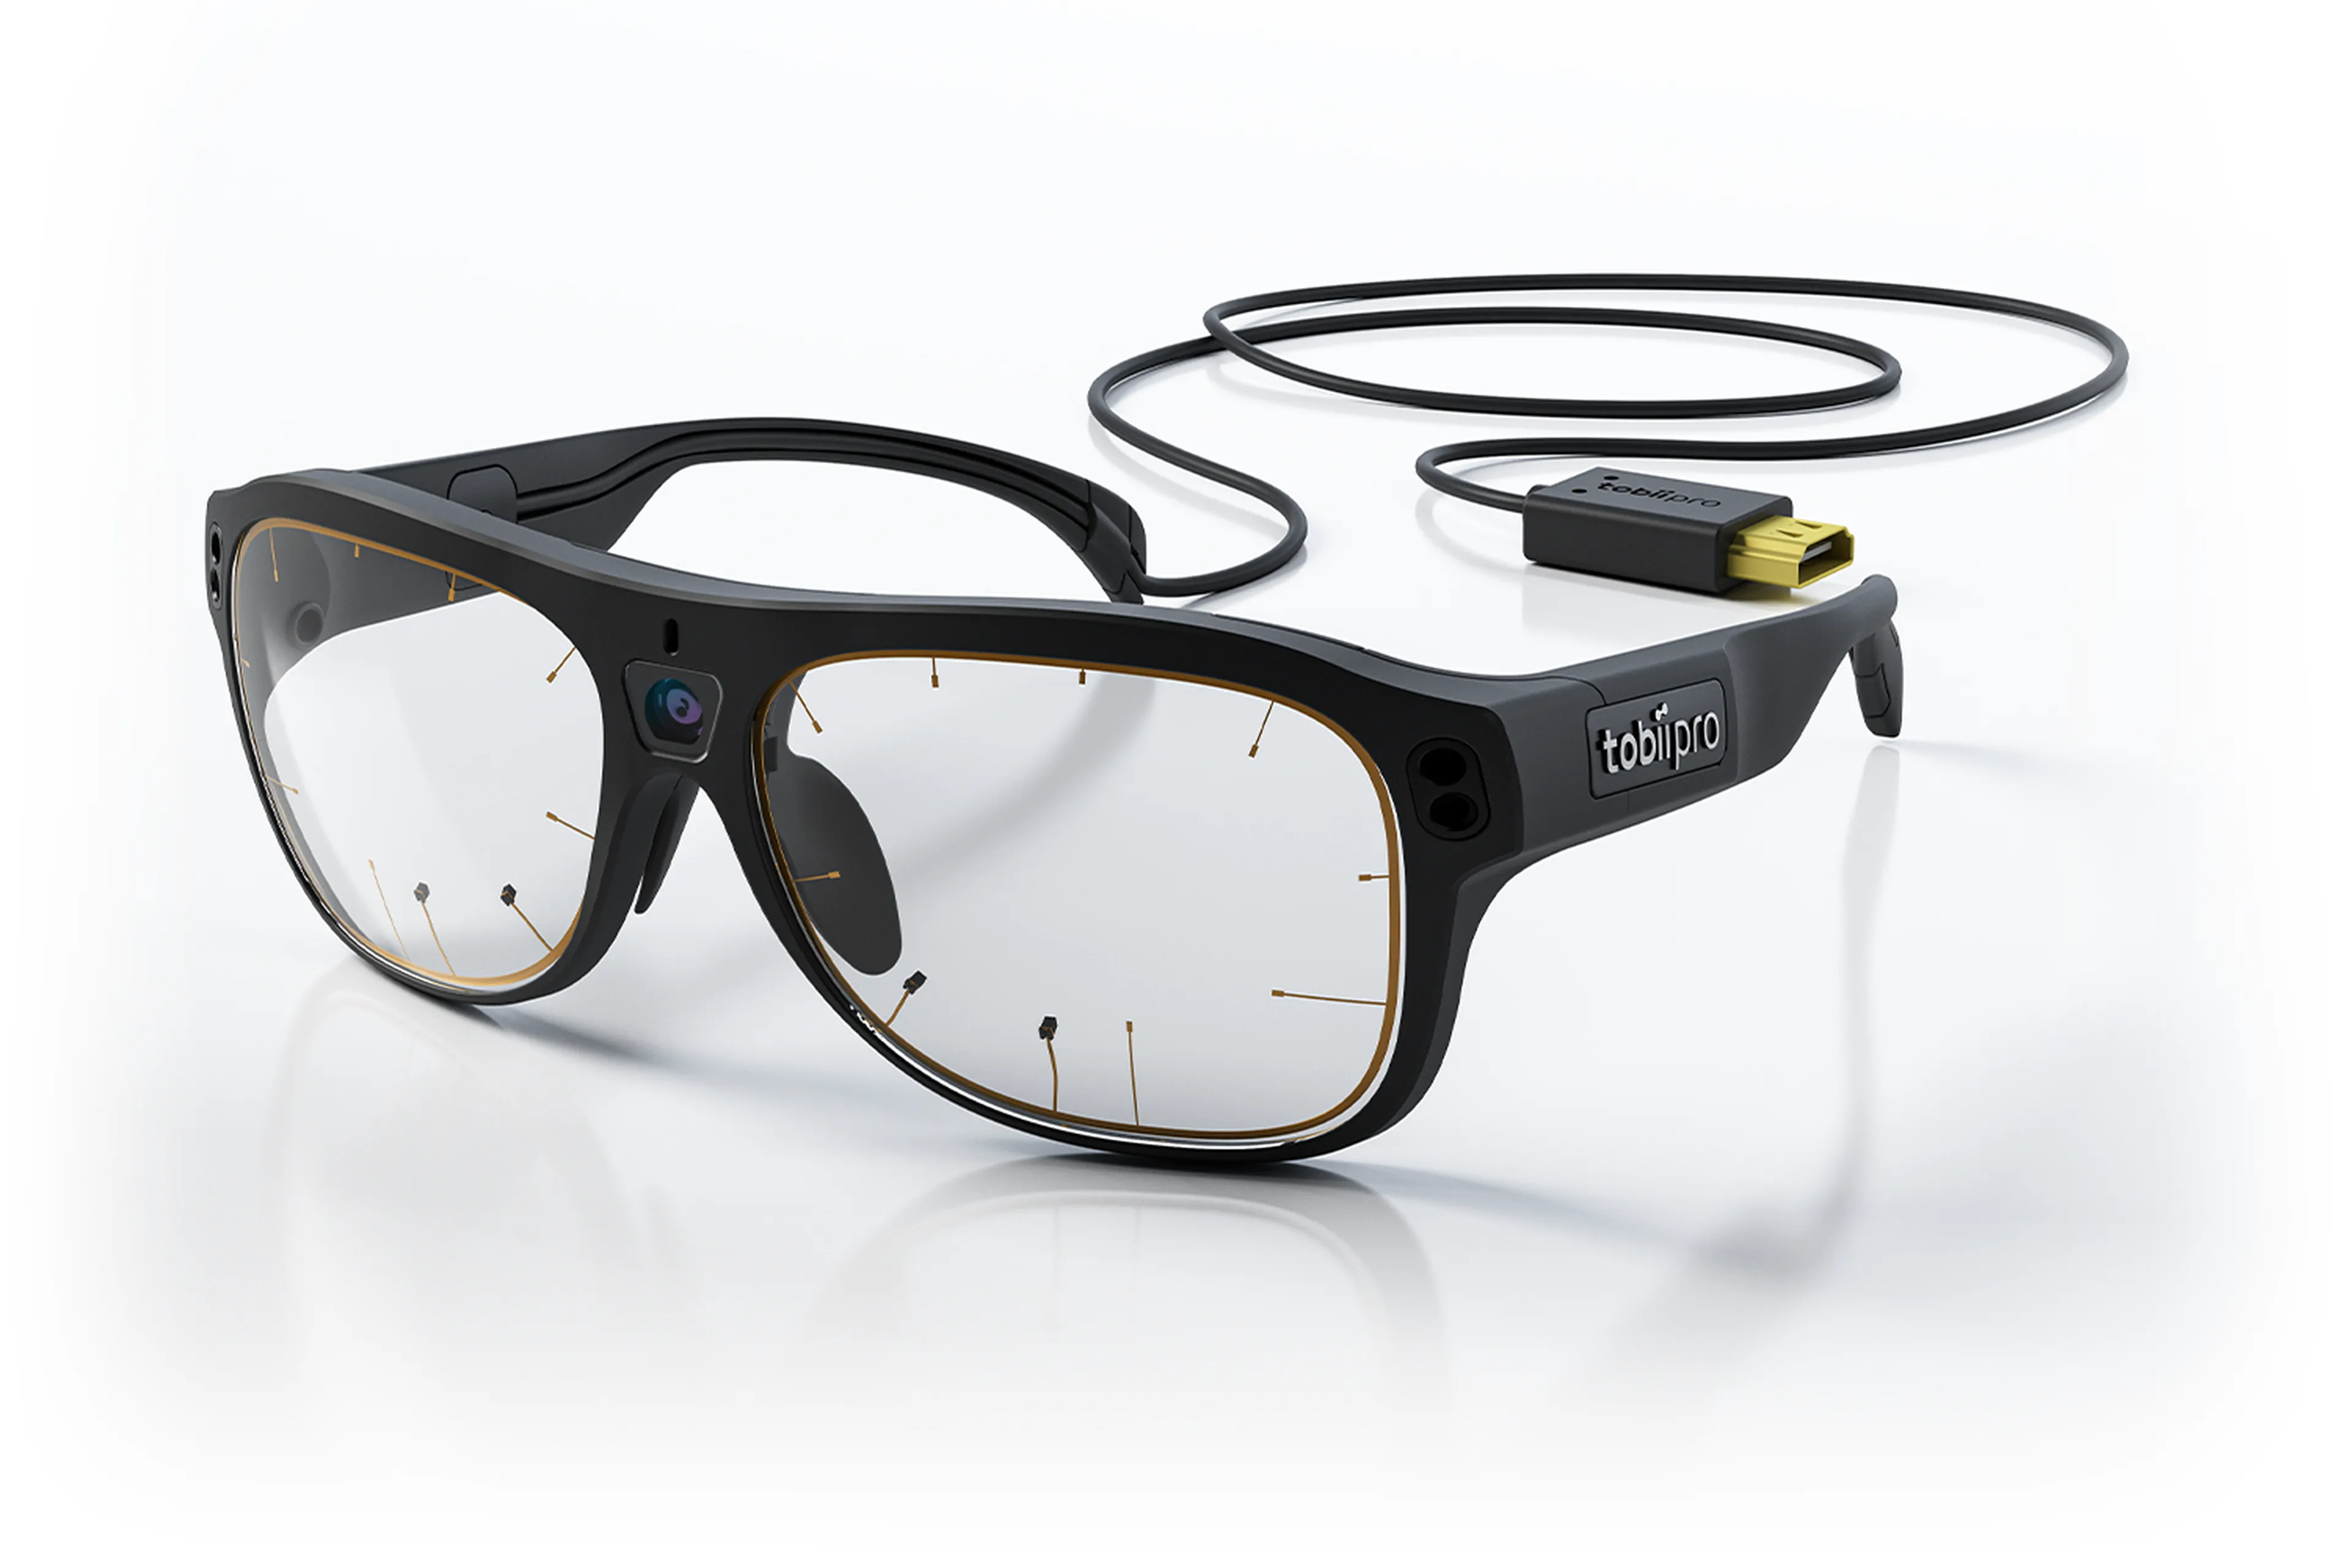
\includegraphics[width=0.5\textwidth]{figuras/tobiiglasses.png}
    \caption{Tobii Glasses}
    \label{fig:tobiiglasses}
\end{figure}

Por otro lado, la empresa \keyword{EyeComTec} desarrolla productos exclusivamente de software como \emph{ECTKeyboard}, \emph{ECTMouse} y \emph{ECTTracker}, que se utilizan para manipular computadoras con tan solo el movimiento de los ojos.

En cuanto a la empresa \keyword{LC Technologies}, cuenta con el sistema \emph{Eyegaze}, un dispositivo con hardware y software propios diseñado para realizar múltiples tareas como navegar por internet, reproducir contenido multimedia, redactar mensajes y controlar dispositivos externos.

También se puede mencionar a \emph{EyeHarp}, un instrumento musical digital que permite tocar música mediante el movimiento de los ojos. Funciona principalmente con rastreadores oculares \emph{Tobii}, aunque también puede utilizarse con otros dispositivos que controlan el puntero del mouse. Está diseñado especialmente para personas con discapacidades físicas o motrices, ofreciendo una forma inclusiva de expresión musical.

A partir de todos estos desarrollos podemos inferir que la tecnología del \emph{eye-tracking} se encuentra sumamente avanzada en el año en el que se realiza este trabajo. Sin embargo, nuestro proyecto se enfoca exclusivamente en el ámbito educativo, y presenta algunas ventajas en relación a estos dispositivos, que se comentarán más adelante.

\section{Motivación}

Todos los ejemplos de sistemas que utilizan \emph{eye-tracking} expuestos anteriormente, ya sea por hardware, software o una combinación de ambos, son herramientas de calidad que pueden aplicarse en una gran variedad de campos. Han aportado una amplia gama de dispositivos versátiles que ayudan tanto a investigaciones científicas y de marketing, como también a facilitar acciones cotidianas.
Sin embargo, el principal problema de estos dispositivos es su alto costo económico. El uso de tecnologías de tan alto nivel implica a su vez altos costos de desarrollo, lo que tiene como consecuencia que muchos de ellos no son accesibles para usuarios en una situación económica desfavorable.
Otro detalle que se pudo observar durante la investigación es que, a pesar de la versatilidad de funcionamiento de estos dispositivos, ninguno está centrado exclusivamente en el ámbito educativo, por lo que se necesita una alternativa más optimizada, intuitiva y sencilla para aplicar en este campo.

Por todo lo anterior expuesto es que se propone este proyecto. Una solución que mantenga la ergonomía y la portabilidad de los dispositivos antes mencionados, sumando a su vez un bajo costo económico, impulsado por el uso de hardware y software de bajos recursos y una orientación exclusiva al ámbito educativo de personas con discapacidades motoras.
Este dispositivo tiene la intención de que pueda ser utilizado en instituciones educativas y familias de escasos recursos, garantizando una accesibilidad mucho mayor a la que cualquier otro dispositivo de alta tecnología pueda ofrecer.


\section{Alcance y objetivos}

El objetivo general de este proyecto es desarrollar un dispositivo de bajo costo basado en microcontroladores económicos que permita a personas con movilidad reducida rendir evaluaciones de opción múltiple y comunicarse mediante seguimiento ocular (\emph{eye-tracking}), funcionando de forma autónoma y sin conexión a internet (\emph{offline}).

Para alcanzar esta meta, se plantean los siguientes objetivos específicos:

\begin{itemize}
    \item Diseñar un dispositivo económico, ergonómico y portable, que funcione sin necesidad de acceso a internet.
    \item Brindar una interfaz intuitiva y de fácil uso, accesible desde cualquier dispositivo con navegador web.
    \item Permitir que los profesores gestionen cuestionarios de opción múltiple personalizados.
    \item Permitir que los tutores realicen un seguimiento académico integral del alumno.
    \item Facilitar un canal de comunicación directo para que docentes, tutores y compañeros puedan realizarle preguntas e interactuar con el estudiante.
    \item Implementar un sistema de registro e inicio de sesión de usuarios, con una base de datos local para el almacenamiento de usuarios, cuestionarios y respuestas.
    \item Realizar el procesamiento de la imagen del ojo del usuario mediante un microcontrolador embebido en el dispositivo.
\end{itemize}

En cuanto al alcance, el proyecto comprende el desarrollo integral de un dispositivo autónomo capaz de capturar la imagen ocular del alumno, procesar la dirección de la mirada y traducir esa información en acciones concretas sobre una interfaz web. El sistema está delimitado para operar en un entorno local, sin depender de conexión a internet ni de infraestructura de red externa, permitiendo el acceso a la plataforma mediante cualquier navegador web compatible.

Respecto a los usuarios del sistema, se delimitan los siguientes roles y permisos:

\begin{itemize}
    \item Alumno: interactúa mediante la mirada para resolver las evaluaciones de opción múltiple y responder a preguntas informales del entorno.
    \item Profesor: encargado de crear, editar y administrar sus cuestionarios académicos.
    \item Tutor: responsable de consultar todos los cuestionarios, junto con las respuestas y los resultados obtenidos por el alumno.
    \item Compañero: habilitado para realizar preguntas esporádicas de opción múltiple con el fin de comunicarse con el alumno, las cuales no quedan registradas en el sistema.
\end{itemize}


